\documentclass{article}
\usepackage[utf8]{inputenc}
\usepackage{geometry}
 \geometry{
 a4paper,
 total={170mm,257mm},
 left=20mm,
 top=20mm,
 }
\usepackage{graphicx}
\usepackage{titling}
\usepackage{enumitem}
\usepackage{float}
\usepackage{caption}
\usepackage{subcaption}
\usepackage{amsmath}
\usepackage{booktabs} % For professional table formatting
\usepackage{appendix}
\usepackage{multirow}
\usepackage{pdfpages} % Package to include PDF pages

\usepackage{hyperref}
\hypersetup{
    colorlinks=true,
    linkcolor=blue,
    filecolor=magenta,      
    urlcolor=cyan,
    pdftitle={Discretization Methods},
    pdfpagemode=FullScreen,
    }

\urlstyle{same}


\title{Take-Home Exam}
\author{Dennys Huber}
\date{\today}
 
 \usepackage{fancyhdr}
\fancypagestyle{plain}{%  the preset of fancyhdr 
    \fancyhf{} % clear all header and footer fields
    \fancyfoot[C]{\thepage}
    % \fancyfoot[L]{\thedate}
    \fancyhead[L]{Discretization Methods}
    \fancyhead[R]{\theauthor}
}
\pagestyle{plain}% Set page style to plain.
\makeatletter
\def\@maketitle{%
  \newpage
  \null
  \vskip 1em%
  \begin{center}%
  \let \footnote \thanks
    {\LARGE \@title \par}%
    \vskip 1em%
    {\large \@author}%
    \vskip 1em%
    {\large \@date}%
  \end{center}%
  \par
  \vskip 1em}
\makeatother


\begin{document}

\maketitle

\section{Advection-Diffusion Equation}\label{sec:advection_diffusion_equation}
The advection-diffusion equation is given as
\begin{equation}
    \frac{\partial u(x,t)}{\partial t} + U_0(x) \frac{\partial u(x,t)}{\partial x} = \nu \frac{\partial^2 u(x,t)}{\partial x^2},
    \label{eq:adv_diff_eq}
\end{equation}
where:
\begin{itemize}
    \item $u(x,t)$ is the unknown function.
    \item $U_0(x)$ is a periodic and bounded velocity field[cite: 304].
    \item $\nu$ is a constant diffusion coefficient[cite: 304].
    \item Both $u(x,t)$ and $U_0(x)$ are assumed to be periodic and smooth, as is the initial condition[cite: 304, 305].
\end{itemize}

\subsection{Sufficient Conditions for Wellposedness}\label{sub:wellposedness}
For Equation \ref{eq:adv_diff_eq} to be wellposed, we need to establish sufficient conditions for $\nu$ and $U_0(x)$.
The problem is considered wellposed for $t \in [0, T]$ in $L^2_w[D]$ provided that its solution $u(\cdot, t)$ satisfies
\begin{equation}
    \|u(\cdot, t)\|_{L_w^2[D]} \leq K e^{\alpha t}\|g\|_{L_w^2[D]},
    \label{eq:wellposed_def}
\end{equation}
for some positive constants $K$ and $\alpha$, where $g$ is the initial condition. \newline
\newline
We establish the following sufficient conditions:
\begin{enumerate}
    \item \textbf{Positive Diffusion Coefficient} $(\nu > 0)$: This coefficient must be strictly positive. A positive $\nu$ ensures that Equation \ref{eq:adv_diff_eq} is parabolic, which is associated with smoothing properties essential for wellposedness. The diffusion term $\nu \frac{\partial^2 u}{\partial x^2}$ introduces dissipation in the energy of the system, which helps to counterbalance potential energy growth from the advection term, as will be shown in the semi-boundedness analysis.
    \item \textbf{Bounded Derivative of} $U_0(x)$: We require $U_0(x)$ to be continuously differentiable, i.e., $U_0(x) \in C^1[0,2\pi]$, with its derivative $U_0'(x)$ being bounded, such that $\max_x|U_0'(x)| < \infty$. This condition ensures that the advection term does not introduce unbounded growth rates in the solution's energy estimate.
\end{enumerate}
%
To demonstrate wellposedness under these conditions, we show that the spatial operator is semi-bounded. The PDE can be written as $\frac{\partial u}{\partial t} = \mathcal{L}u$, where the spatial operator $\mathcal{L}$ is defined as:
\begin{equation}
    \mathcal{L} = - U_0(x) \frac{\partial}{\partial x} + \nu \frac{\partial^2}{\partial x^2}.
    \label{eq:oper_semi_bound}
\end{equation}
To find the adjoint $\mathcal{L}^*$, we use the $L^2[0, 2\pi]$ inner product $(f,g)_{L^2} = \int_0^{2\pi} f(x) \overline{g(x)} dx$. The adjoint $\mathcal{L}^*$ is defined by $(\mathcal{L}u, v)_{L^2} = (u, \mathcal{L}^*v)_{L^2}$ for all sufficiently smooth $u,v$ satisfying periodic boundary conditions.
\begin{equation}
    (\mathcal{L}u, v)_{L^2} = \int_0^{2\pi} \left( -U_0(x) \frac{\partial u}{\partial x} + \nu \frac{\partial^2 u}{\partial x^2} \right) v dx.
    \label{eq:adjoint_l_star_integral}
\end{equation}
Analyzing the terms individually:
\begin{itemize}
    \item \textbf{Advection term}: Using integration by parts:
          \begin{equation}
              \int_0^{2\pi} - U_0 (x) \frac{\partial u}{\partial x} v dx = \left [ -U_0(x) u v \right]_0^{2\pi} + \int_0^{2\pi} u \frac{\partial}{\partial x} \left ( U_0(x) v\right) dx.
              \label{eq:adv_term_parts}
          \end{equation}
          The boundary term $\left [ -U_0(x) u v \right]_0^{2\pi}$ vanishes due to the periodicity of $U_0(x)$, $u(x,t)$, and the test function $v(x)$ over $[0, 2\pi]$. The remaining term is expanded as:
          \begin{equation}
              \int_0^{2\pi} u \frac{\partial}{\partial x} \left ( U_0(x) v\right) dx = \int_0^{2\pi} u \left ( U_0(x) \frac{dv}{dx} +  \frac{d U_0(x)}{d x} v \right) dx.
              \label{eq:adv_term_expanded}
          \end{equation}
          So, the adjoint of $-U_0(x) \frac{\partial}{\partial x}$ is $U_0(x) \frac{\partial}{\partial x} + \frac{d U_0(x)}{dx}$.
    \item \textbf{Diffusion term}: Applying integration by parts twice:
          \begin{equation}
              \begin{aligned}
                  \int_0^{2 \pi} \nu \frac{\partial^2 u }{\partial x^2} v dx & = \underbrace{\left [ \nu \frac{\partial u}{\partial x} v \right]_0^{2\pi}}_{=0, \text{ due to periodicity}} - \int_0^{2\pi} \nu \frac{\partial u}{\partial x} \frac{\partial v}{\partial x} dx \\
                                                                         & =  \underbrace{\left [ -\nu u \frac{\partial v}{\partial x} \right]_0^{2\pi}}_{=0, \text{ due to periodicity}} + \int_0^{2\pi} \nu u \frac{\partial^2 v}{\partial x^2} dx.
                  \label{eq:diff_term_parts}
              \end{aligned}
          \end{equation}
          Thus, the diffusion operator $\nu \frac{\partial^2}{\partial x^2}$ is self-adjoint under periodic boundary conditions.
\end{itemize}
Combining these results, we have:
\begin{equation}
    (\mathcal{L}u , v )_{L^2} =  \int_0^{2\pi} u \left ( U_0(x) \frac{\partial v}{\partial x} +  \frac{d U_0(x)}{d x} v  +  \nu \frac{\partial^2 v}{\partial x^2} \right) dx = (u, \mathcal{L}^* v)_{L^2}.
    \label{eq:adj_eq_final}
\end{equation}
Therefore, the adjoint operator is:
\begin{equation}
    \mathcal{L}^* = U_0(x) \frac{\partial}{\partial x} +  \frac{d U_0(x)}{d x}  +  \nu \frac{\partial^2}{\partial x^2}.
    \label{eq:adj_op_final}
\end{equation}
An operator $\mathcal{L}$ is semi-bounded if there exists a real constant $\alpha$ such that for all $u$ in the domain of $\mathcal{L}$:
\begin{equation}
    \left(u,\left(\mathcal{L}+\mathcal{L}^*\right) u\right)_{L^2} \leq \alpha\|u\|_{L^2}^2 \quad \text{or equivalently } \text{Re}(\mathcal{L}u, u)_{L^2} \leq \frac{\alpha}{2} \|u\|_{L^2}^2 \text{}.
    \label{eq:semi_bounded_def}
\end{equation}
First, we compute $\mathcal{L} + \mathcal{L}^*$:
\begin{equation}
    \mathcal{L} + \mathcal{L}^* = \left (  - U_0(x) \frac{\partial}{\partial x} + \nu \frac{\partial^2}{\partial x^2} \right) + \left  (U_0(x) \frac{\partial}{\partial x} +  \frac{d U_0(x)}{d x}  +  \nu \frac{\partial^2}{\partial x^2} \right ) = \frac{d U_0(x)}{d x}  +  2\nu \frac{\partial^2}{\partial x^2}.
    \label{eq:L_plus_L_star}
\end{equation}
Using this result, we compute the inner product:
\begin{equation}
    \begin{aligned}
        (u, (\mathcal{L}+\mathcal{L}^*)u)_{L^2} & = \int_0^{2\pi} u\left(\frac{dU_0(x)}{dx}u + 2\nu\frac{\partial^2 u}{\partial x^2}\right) dx  \\
                                               & = \int_0^{2\pi} \frac{dU_0(x)}{dx}u^2 dx + 2\nu\int_0^{2\pi} u\frac{\partial^2 u}{\partial x^2} dx.
    \end{aligned}
    \label{eq:uLLu_expanded}
\end{equation}
For the second term, integration by parts (and using periodicity of $u$ and its derivatives) yields, for $\nu > 0$:
\begin{equation}
    2 \nu \int_0^{2 \pi} u \frac{\partial^2 u}{\partial x^2} dx = \underbrace{2\nu \left[u \frac{\partial u}{\partial x}\right]_0^{2\pi}}_{=0} - 2 \nu \int_0^{2 \pi} \left (\frac{\partial u}{\partial x} \right )^2 dx  \leq 0.
    \label{eq:diff_term_energy}
\end{equation}
This non-positive contribution from the diffusion term is key for stability if $U_0'(x)$ can be negative. This leads to:
\begin{equation}
    (u, (\mathcal{L}+\mathcal{L}^*)u)_{L^2} \leq \int_0^{2\pi} \frac{dU_0(x)}{dx}u^2 dx \leq  \max_x\left|\frac{dU_0(x)}{dx}\right| \int_0^{2\pi} u^2 dx = \max_x\left|\frac{dU_0(x)}{dx}\right| \|u\|^2_{L^2}.
    \label{eq:wellposed_cond_deriv}
\end{equation}
Thus, the condition for semi-boundedness (\ref{eq:semi_bounded_def}) is satisfied with
\begin{equation}
    \alpha = \max_x\left|\frac{dU_0(x)}{dx}\right|.
    \label{eq:alpha_val}
\end{equation}
This is satisfied if $U_0(x)$ has a bounded derivative, as per our condition 2.
According to the theorem relating semi-boundedness to wellposedness (e.g., HGG p.52, for Gale, if operator $\mathcal{L}$ is semi-bounded, then the Initial Boundary Value Problem (IBVP) is wellposed in an energy sense, yielding:
\begin{equation}
    \frac{d}{d t}\|u\|_{L^2}^2 \leq \alpha\|u\|_{L^2}^2 \Rightarrow\|u(t)\|_{L^2}^2 \leq e^{\alpha t}\|u(0)\|_{L^2}^2.
    \label{eq:wellposed_result}
\end{equation}

\textbf{Summary of Sufficient Conditions}: The problem is wellposed if:
\begin{itemize}
    \item $\nu > 0$ (strictly positive diffusion coefficient).
    \item $U_0(x) \in C^1[0,2\pi]$ with its derivative $\frac{dU_0(x)}{dx}$ bounded.
\end{itemize}
% subsection Wellposedness (end)

\subsection{Consistency and Convergence Rate of Fourier Collocation Approximation}\label{sub:consistency_and_convergence_rate_of_fourier_collocation_approximation}

The Fourier Collocation method approximates the solution $u(x,t)$ using a truncated Fourier series:
\begin{equation}
u_N(x,t) = \sum_{k=-N/2}^{N/2} \tilde{u}_k(t) e^{ikx},
\label{eq:fourier_approx}
\end{equation}
where the coefficients $\tilde{u}_k(t)$ are determined by satisfying the PDE at a set of collocation points $x_j$.

\subsubsection{Consistency Analysis}
An approximation is consistent if the truncation error tends to zero as $N \rightarrow \infty$. More formally, for the scheme $\frac{\partial u_N}{\partial t} = \mathcal{L}_N u_N = P_N \mathcal{L} P_N u_N$, consistency requires:
\begin{equation}
\|P_N \mathcal{L}(I - P_N)u\|_{L^2} \rightarrow 0 \text{ as } N \rightarrow \infty,
\label{eq:consistency_cond1}
\end{equation}
and that the approximation of the initial condition is also consistent:
\begin{equation}
\|P_N u(0) - u_N(0)\|_{L^2} \rightarrow 0 \text{ as } N \rightarrow \infty,
\label{eq:consistency_cond2}
\end{equation}
where $u$ is the exact solution and $P_N$ is the projection operator onto the space of trigonometric polynomials of degree up to $N/2$.
For the advection-diffusion equation, the operator is $\mathcal{L} = -U_0(x)\frac{\partial}{\partial x} + \nu\frac{\partial^2}{\partial x^2}$.
\begin{enumerate}
    \item \textbf{Smoothness and Periodicity}: Given that $u(x,t)$ and $U_0(x)$ are smooth ($C^\infty$) and periodic, their product $U_0(x)u(x,t)$ is also $C^\infty$ and periodic. Derivatives of $C^\infty$ periodic functions, such as $\frac{\partial u}{\partial x}$ and $\frac{\partial^2 u}{\partial x^2}$, are also $C^\infty$ and periodic.
    \item \textbf{Fourier Coefficient Decay}: For a $C^\infty$ periodic function $f(x)$, its Fourier coefficients $\hat{f}_k$ decay faster than any algebraic power of $|k|$ (i.e., $|\hat{f}_k| = o(|k|^{-m})$ for all $m > 0$), which is often referred to as spectral or exponential decay. Thus, the Fourier coefficients of $U_0(x)\frac{\partial u}{\partial x}$ and $\nu\frac{\partial^2 u}{\partial x^2}$ exhibit such rapid decay.
    \item \textbf{Truncation Error Term $(I-P_N)u$}: The error in approximating a $C^\infty$ periodic function $u$ by its truncated Fourier series $P_N u$, which is $u - P_N u = (I-P_N)u$, also decays spectrally in appropriate norms. For instance, $||u - P_N u||_{L^2}$ decays spectrally.
    \item \textbf{Action of $\mathcal{L}$ on $(I-P_N)u$}: Since $(I-P_N)u$ is a sum of high-frequency modes and decays rapidly, applying the differential operator $\mathcal{L}$ (which involves derivatives and multiplication by a smooth function $U_0(x)$) to $(I-P_N)u$ will result in a function whose Fourier coefficients also decay rapidly. While differentiation amplifies higher frequencies (multiplying coefficients by $ik$ or $(ik)^2$), if the original decay is sufficiently fast (e.g., exponential), the result $\mathcal{L}(I-P_N)u$ will still tend to zero rapidly as $N \rightarrow \infty$.
    \item \textbf{Projection $P_N$}: Applying the projector $P_N$ to $\mathcal{L}(I-P_N)u$ does not alter its convergence to zero.
\end{enumerate}
Therefore, the condition $\|P_N \mathcal{L}(I - P_N)u\|_{L^2} \rightarrow 0$ as $N \rightarrow \infty$ is satisfied. Assuming the initial condition $u_N(0)$ is chosen as $P_N u(x,0)$, the second condition for consistency is also met. Thus, the Fourier Collocation method is consistent for this problem under the given smoothness assumptions.

\subsubsection{Expected Convergence Rate}
The convergence rate of the Fourier Collocation method is determined by how well the truncated Fourier series can approximate the true solution. Given the smoothness and periodicity assumptions from the problem statement:

\textbf{For infinitely smooth ($C^\infty$) periodic functions}:
\begin{itemize}
    \item The Fourier coefficients $\hat{u}_n$ of $u(x,t)$ decay faster than any polynomial power of $|n|$, often exponentially, e.g., $|\hat{u}_n| \sim e^{-\alpha|n|}$ for some $\alpha > 0$.
    \item This rapid decay leads to \textbf{spectral convergence} (often exponential convergence) for the approximation error. For the $L^2$ norm, $||u - u_N||_{L^2} \sim e^{-\beta N}$ for some $\beta > 0$.
    \item This means the error decreases faster than any fixed polynomial rate $N^{-p}$ as $N$ increases.
\end{itemize}

\textbf{For functions with limited regularity} (e.g., $u \in C^m[0,2\pi]$ and all derivatives up to $m-1$ are periodic):
\begin{itemize}
    \item The Fourier coefficients satisfy $|\hat{u}_n| \sim O(|n|^{-m})$ for large $|n|$.
    \item This leads to an \textbf{algebraic convergence rate} for the approximation error, typically $||u - u_N||_{L^2} \sim O(N^{-m})$.
    \item This is still significantly faster than typical low-order finite difference methods, which might achieve $O(N^{-p})$ where $p$ is a small integer (e.g., 2 or 4).
\end{itemize}


% subsection Consistency and Convergence Rate of Fourier Collocation Approximation (end)

\subsection{Stability of Fourier Collocation for Constant $U_0$}\label{sub:stability_constant_u0}

When $U_0(x) = U_0$ (a constant), the advection-diffusion equation (\ref{eq:adv_diff_eq}) simplifies to:
\begin{equation}
\frac{\partial u}{\partial t} + U_0 \frac{\partial u}{\partial x} = \nu \frac{\partial^2 u}{\partial x^2}.
\label{eq:adv_diff_const_U0}
\end{equation}
We aim to prove the stability of the semi-discrete approximation obtained using the Fourier Collocation method with an odd number of modes ($N+1$ grid points, where $N$ is even).

\subsubsection{Semi-discrete Formulation}
The semi-discrete system, obtained by applying Fourier collocation in space, can be written in vector form as:
\begin{equation}
\frac{d\mathbf{u}}{dt} = -U_0 \tilde{D} \mathbf{u} + \nu \tilde{D}^{(2)} \mathbf{u},
\label{eq:semidiscrete_const_U0}
\end{equation}
where:
\begin{itemize}
    \item $\mathbf{u}(t) = [u(x_0,t), u(x_1,t), \ldots, u(x_N,t)]^T$ is the vector of solution values at the $N+1$ collocation points $x_j = \frac{2\pi j}{N+1}$ for $j=0, \dots, N$.
    \item $\tilde{D}$ is the $(N+1) \times (N+1)$ first-order Fourier collocation differentiation matrix. For the odd number of points, this matrix is real and skew-symmetric, i.e., $\tilde{D}^T = -\tilde{D}$.
    \item $\tilde{D}^{(2)}$ is the second-order Fourier collocation differentiation matrix. For the odd method, $\tilde{D}^{(2)} = \tilde{D}^2$. Since $\tilde{D}$ is skew-symmetric, $\tilde{D}^2 = \tilde{D}(-\tilde{D}^T) = -\tilde{D}\tilde{D}^T$, which is a symmetric and negative semi-definite matrix.
\end{itemize}

\subsubsection{Energy Method Proof}
We define the discrete energy (squared $L^2$-norm analogue) as:
\begin{equation}
E(t) = \frac{1}{N+1} \sum_{j=0}^{N} |u_j(t)|^2 = \frac{1}{N+1} \mathbf{u}(t)^T \mathbf{u}(t),
\label{eq:discrete_energy}
\end{equation}
assuming $u_j(t)$ are real, which is consistent with $u(x,t)$ being a real-valued solution.
Taking the time derivative of $E(t)$:
\begin{equation}
\frac{dE}{dt} = \frac{1}{N+1} \left( \frac{d\mathbf{u}^T}{dt}\mathbf{u} + \mathbf{u}^T\frac{d\mathbf{u}}{dt} \right) = \frac{2}{N+1} \mathbf{u}^T \frac{d\mathbf{u}}{dt}
\label{eq:dEdt_general}
\end{equation}
(since $\mathbf{u}^T \frac{d\mathbf{u}}{dt}$ is a scalar, it equals $\text{Re}(\mathbf{u}^T \frac{d\mathbf{u}}{dt})$).
Substituting the semi-discrete equation (\ref{eq:semidiscrete_const_U0}):
\begin{equation}
\begin{aligned}
\frac{dE}{dt} &= \frac{2}{N+1} \mathbf{u}^T (-U_0 \tilde{D} \mathbf{u} + \nu \tilde{D}^{(2)} \mathbf{u}) \\
&= -\frac{2U_0}{N+1} (\mathbf{u}^T \tilde{D} \mathbf{u}) + \frac{2\nu}{N+1} (\mathbf{u}^T \tilde{D}^{(2)} \mathbf{u}).
\end{aligned}
\label{eq:dEdt_substituted}
\end{equation}
We analyze each term:
\begin{enumerate}
    \item \textbf{Advection term}: $\mathbf{u}^T \tilde{D} \mathbf{u}$. Since $\tilde{D}$ is skew-symmetric ($\tilde{D}^T = -\tilde{D}$) and $\mathbf{u}$ is real:
        \begin{equation}
        \mathbf{u}^T \tilde{D} \mathbf{u} = (\mathbf{u}^T \tilde{D} \mathbf{u})^T = \mathbf{u}^T \tilde{D}^T \mathbf{u} = \mathbf{u}^T (-\tilde{D}) \mathbf{u} = -\mathbf{u}^T \tilde{D} \mathbf{u}.
        \end{equation}
        This implies $2 \mathbf{u}^T \tilde{D} \mathbf{u} = 0$, so $\mathbf{u}^T \tilde{D} \mathbf{u} = 0$. Thus, the advection term contributes nothing to the energy growth.
    \item \textbf{Diffusion term}: $\mathbf{u}^T \tilde{D}^{(2)} \mathbf{u}$. For the odd method, $\tilde{D}^{(2)} = \tilde{D}^2$. Since $\tilde{D}$ is real and skew-symmetric:
        \begin{equation}
        \mathbf{u}^T \tilde{D}^2 \mathbf{u} = \mathbf{u}^T \tilde{D} (-\tilde{D}^T) \mathbf{u} = - (\tilde{D}^T\mathbf{u})^T (\tilde{D}^T\mathbf{u}) = -\|\tilde{D}^T\mathbf{u}\|_2^2.
        \end{equation}
        Since $||\tilde{D}^T\mathbf{u}||_2^2 = ||-\tilde{D}\mathbf{u}||_2^2 = ||\tilde{D}\mathbf{u}||_2^2 \ge 0$, we have $\mathbf{u}^T \tilde{D}^2 \mathbf{u} = -\|\tilde{D}\mathbf{u}\|_2^2 \leq 0$.
\end{enumerate}
Therefore, Equation \ref{eq:dEdt_substituted} becomes:
\begin{equation}
\frac{dE}{dt} = \frac{2\nu}{N+1} (-||\tilde{D}\mathbf{u}\|_2^2) \leq 0,
\label{eq:dEdt_final}
\end{equation}
since $\nu > 0$ (a sufficient condition for wellposedness derived earlier).
This proves that the discrete energy $E(t)$ is non-increasing ($E(t) \le E(0)$), establishing the \textbf{unconditional stability} of the semi-discrete Fourier Collocation approximation in the discrete $L^2$-norm analogue.

% \subsubsection{Alternative Proof via Fourier Analysis}
% Let $u_N(x,t) = \sum_{n=-N/2}^{N/2} \hat{u}_n(t) e^{inx}$ be the Fourier series representation of the solution (here, $\hat{u}_n$ denote the time-dependent Fourier coefficients, equivalent to $\tilde{u}_n$ used earlier).
% Applying this to Equation \ref{eq:adv_diff_const_U0}, and noting that $e^{inx}$ are eigenfunctions of the Fourier differentiation operators:
% $\frac{\partial}{\partial x} (e^{inx}) = in e^{inx}$ and $\frac{\partial^2}{\partial x^2} (e^{inx}) = (in)^2 e^{inx} = -n^2 e^{inx}$.
% The PDE transforms into a system of ODEs for each mode $\hat{u}_n(t)$:
% \begin{equation}
% \frac{d\hat{u}_n(t)}{dt} + U_0 (in \hat{u}_n(t)) = \nu (-n^2 \hat{u}_n(t)).
% \end{equation}
% Thus,
% \begin{equation}
% \frac{d\hat{u}_n(t)}{dt} = -(inU_0 + n^2\nu)\hat{u}_n(t).
% \label{eq:modal_ode}
% \end{equation}
% The solution to this ODE is:
% \begin{equation}
% \hat{u}_n(t) = \hat{u}_n(0) e^{-(inU_0 + n^2\nu)t}.
% \label{eq:modal_solution}
% \end{equation}
% The magnitude of each coefficient evolves as:
% \begin{equation}
% |\hat{u}_n(t)| = |\hat{u}_n(0) e^{-inU_0 t} e^{-n^2\nu t}| = |\hat{u}_n(0)| |e^{-inU_0 t}| |e^{-n^2\nu t}| = |\hat{u}_n(0)| e^{-n^2\nu t}.
% \label{eq:modal_magnitude}
% \end{equation}
% Since $\nu > 0$ (from the wellposedness conditions) and $n^2 \ge 0$, the term $e^{-n^2\nu t} \leq 1$ for all $t \ge 0$.
% Therefore, $|\hat{u}_n(t)| \leq |\hat{u}_n(0)|$ for each mode $n$.
% By Parseval's identity for the $L^2[0, 2\pi]$ norm:
% \begin{equation}
% \|u_N(t)\|_{L^2}^2 = 2\pi \sum_{n=-N/2}^{N/2} |\hat{u}_n(t)|^2 \leq 2\pi \sum_{n=-N/2}^{N/2} |\hat{u}_n(0)|^2 = \|u_N(0)\|_{L^2}^2.
% \label{eq:parseval_stability}
% \end{equation}
% This shows that the $L^2$-norm of the solution does not grow in time, confirming unconditional stability.
%
% subsection Stability of Fourier Collocation for Constant U_0 (end)

\section{Solving Burger's Equation using Fourier Collocation}
The Fourier Collocation method was implemented using odd-numbered grid points defined as:
\begin{equation}
	x_j = \frac{2\pi}{N+1}j, \quad j \in [0, N]
\end{equation}
The Spatial derivatives were computed using the Fourier differentiation matrix $\tilde{D}$, and time integration was performed using the 4th-order Runge-Kutta scheme.
\begin{equation}
	\begin{align}
		u_1     & = u^n + \frac{\Delta t}{2}F(u^n)                                             \\
		u_2     & = u^n + \frac{\Delta t}{2}F(u_1)                                             \\
		u_3     & = u^n + \Delta t F(u_2)                                                      \\
		u^{n+1} & = \frac{1}{3}\left[-u^n + u_1 + 2u_2 + u_3 + \frac{\Delta t}{2}F(u_3)\right]
	\end{align}
	\label{eq:rk4_burgers}
\end{equation}
where $F(u^n) = -u^n\frac{\partial u^n}{\partial x} + \nu\frac{\partial^2 u^n}{\partial x^2}$.\newline
The time step was determined according to the following CFL condition
\begin{equation}
	\Delta t \leq \text{CFL} \times \left[\max_{x_j} \left(\frac{|u(x_j)|}{\Delta x} + \frac{\nu}{(\Delta x)^2}\right) \right]^{-1}
\end{equation}

\subsection{Determining Maximum CFL Values}

\subsubsection{Methodology}
The maximum stable CFL values were determined through an incremental testing approach that systematically explores the stability boundary for each grid size. The algorithm proceeds as follows:

\begin{enumerate}
	\item \textbf{Incremental Testing}: For each grid size $N$, CFL values are tested incrementally starting from 0.05 with steps of 0.05
	\item \textbf{Stability Criterion}: A solution is considered stable if:
	      \begin{itemize}
		      \item No NaN or infinite values occur during time integration
		      \item The error change between consecutive CFL values satisfies: $|\text{error}_{\text{current}} - \text{error}_{\text{previous}}| < 0.25$
	      \end{itemize}
	\item \textbf{Termination}: Testing stops when the stability criterion is violated, indicating the onset of numerical instability
	\item \textbf{Safety Selection}: The last stable CFL value is selected as the maximum for practical use
\end{enumerate}

This methodology is theoretically sound as it detects the transition from stable to unstable numerical behavior through the characteristic sharp increase in $L_\infty$ error that occurs at the stability boundary.

\begin{figure}[H]
	\begin{center}
		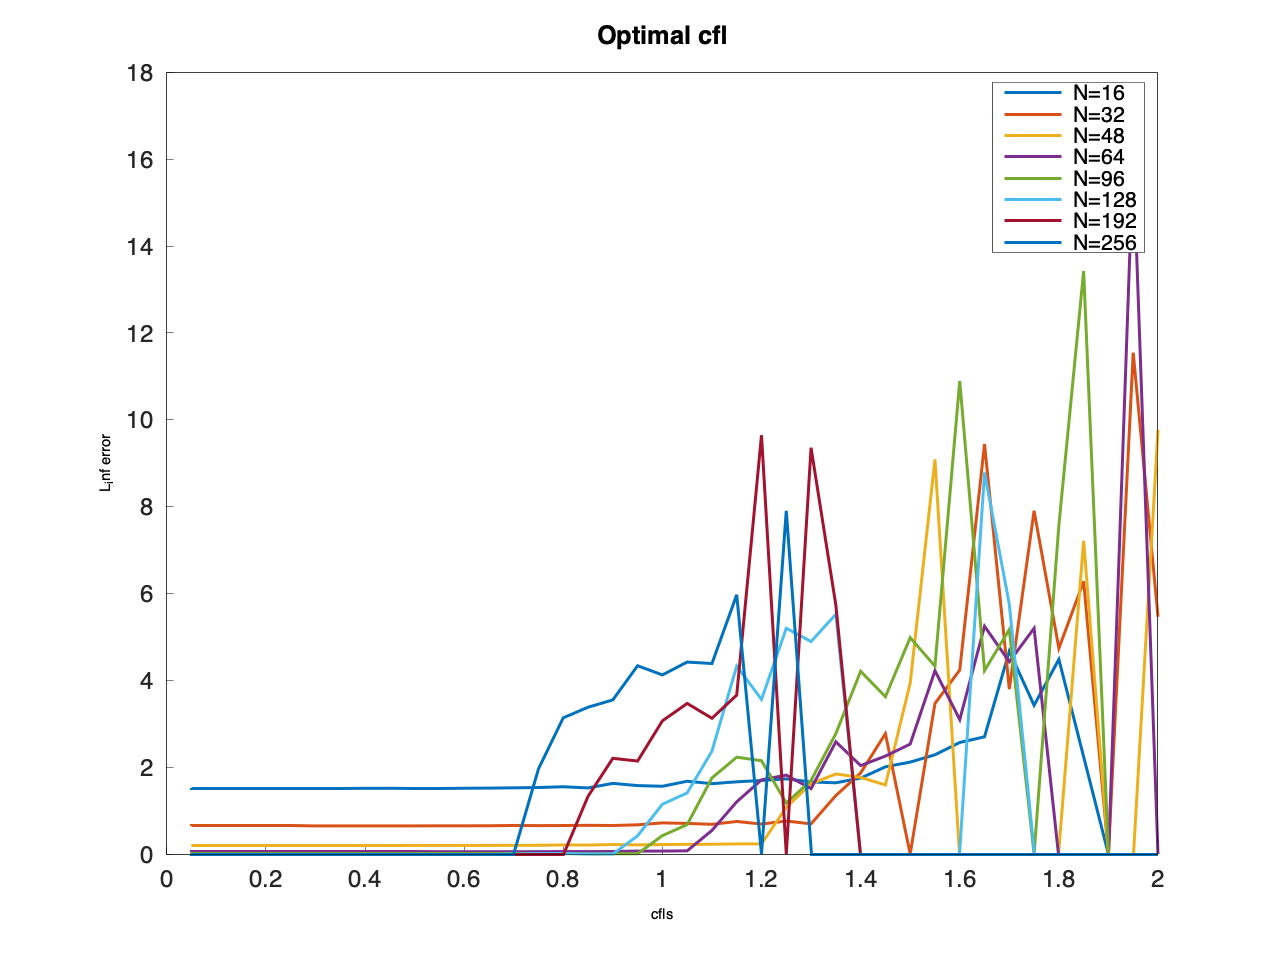
\includegraphics[width=0.5\textwidth]{media/cfl_errors.png}
	\end{center}
	\caption{$L_{\infty}$ error for different CFL values and grid sizes. The sharp spikes in error indicate the onset of numerical instability, which occurs at progressively smaller CFL values as the grid is refined. This behavior correctly identifies the stability limits for each grid resolution.}\label{fig:error_fc}
\end{figure}

\begin{table}[H]
	\centering
	\begin{tabular}{|c|c|}
		\hline
		$N$ & Max CFL \\
		\hline
		16  & 1.4000  \\
		32  & 1.2500  \\
		48  & 1.1500  \\
		64  & 1.0000  \\
		96  & 0.9500  \\
		128 & 0.9000  \\
		192 & 0.7500  \\
		256 & 0.6500  \\
		\hline
	\end{tabular}
	\caption{Maximum stable CFL values for different grid sizes}
	\label{tab:cfl}
\end{table}

\subsubsection{Analysis of CFL Results}
The maximum CFL values exhibit a clear decreasing trend with increasing grid resolution, which is both expected and theoretically correct. This behavior can be explained through the CFL stability condition:

\begin{itemize}
	\item \textbf{Grid Refinement Effect}: As $N$ increases, $\Delta x = \frac{2\pi}{N+1}$ decreases proportionally
	\item \textbf{Diffusion Dominance}: For fine grids, the diffusion constraint $\frac{\nu}{(\Delta x)^2}$ becomes dominant, scaling as $\frac{1}{(\Delta x)^2}$
	\item \textbf{Stability Restriction}: This quadratic dependence on grid spacing makes the time step constraint increasingly restrictive for finer grids
\end{itemize}

The observed CFL values are higher than the typical limit of $\approx 0.5$ for pure diffusion problems because Burgers' equation combines both advection and diffusion effects, with the advection term allowing for larger stable time steps, particularly on coarser grids.

\subsection{Convergence Study}
\begin{table}[H]
	\centering
	\begin{tabular}{|c|c|c|c|}
		\hline
		$N$ & CFL    & $L_\infty$ Error & CPU Time \\
		\hline
		16  & 1.4000 & 9.912532e-01     & 0.0050s  \\
		32  & 1.2500 & 3.440127e-01     & 0.0081s  \\
		48  & 1.1500 & 1.467597e-01     & 0.0142s  \\
		64  & 1.0000 & 2.399181e-02     & 0.0219s  \\
		96  & 0.9500 & 3.176611e-03     & 0.0371s  \\
		128 & 0.9000 & 2.522970e-04     & 0.0573s  \\
		192 & 0.7500 & 1.511961e-05     & 0.1158s  \\
		256 & 0.6500 & 1.657833e-06     & 0.2190s  \\
		\hline
	\end{tabular}
	\caption{Convergence study results for different grid sizes at $t = \pi/4$}
	\label{tab:convergence}
\end{table}

\begin{table}[H]
	\centering
	\begin{tabular}{|c|c|}
		\hline
		$N$ & Rate \\
		\hline
		32  & 1.53 \\
		48  & 2.10 \\
		64  & 6.30 \\
		96  & 4.99 \\
		128 & 8.80 \\
		192 & 6.94 \\
		256 & 7.68 \\
		\hline
	\end{tabular}
	\caption{Convergence rates between successive grid refinements}
	\label{tab:rates}
\end{table}

\subsubsection{Convergence Analysis}
The convergence study reveals \textbf{spectral convergence}, which is the hallmark of Fourier spectral methods applied to smooth, periodic functions:

\begin{itemize}
	\item \textbf{High-Order Rates}: Convergence rates consistently exceed 2, with many values between 6-8, indicating convergence faster than any fixed polynomial order
	\item \textbf{Spectral Theory}: For $C^\infty$ periodic functions, Fourier coefficients decay exponentially as $|\hat{u}_n| \sim e^{-\alpha|n|}$, leading to spectral convergence
	\item \textbf{Rate Variability}: The variation in convergence rates (rather than a constant algebraic rate) is characteristic of the transition between different accuracy regimes in spectral methods
	\item \textbf{Physical Validation}: The high convergence rates confirm that the Burgers' solution remains smooth and well-resolved at $t = \pi/4$
\end{itemize}

This behavior demonstrates that the Fourier Collocation method is exploiting the full smoothness of the solution, achieving the optimal convergence rate possible for this class of problems.

\subsection{Time Evolution Study}
\begin{table}[H]
	\centering
	\begin{tabular}{|c|c|c|}
		\hline
		Time   & $L_\infty$ Error & CPU Time \\
		\hline
		0.0000 & 0.000000e+00     & 0.0000s  \\
		0.3927 & 9.544388e-04     & 0.0314s  \\
		0.5236 & 6.480862e-04     & 0.0421s  \\
		0.7854 & 2.522970e-04     & 0.0651s  \\
		\hline
	\end{tabular}
	\caption{Time evolution for N = 128 with $\nu = 0.10$ and CFL = 0.90}
	\label{tab:time_evolution}
\end{table}

\subsubsection{Error Evolution Analysis}
The time evolution study reveals a counterintuitive but physically correct phenomenon: \textbf{the numerical error decreases over time} from $t = \pi/8$ to $t = \pi/4$. This behavior can be explained through the physics of the viscous Burgers' equation:

\begin{itemize}
	\item \textbf{Viscous Smoothing}: The diffusion term $\nu\frac{\partial^2 u}{\partial x^2}$ acts as a smoothing mechanism, gradually reducing sharp gradients in the solution
	\item \textbf{Initial Complexity}: Early in the evolution ($t = \pi/8$), the solution may contain steeper gradients or transitional features that are more challenging to resolve numerically
	\item \textbf{Fourier Advantage}: As the solution becomes smoother due to viscous effects, it is better represented by the truncated Fourier series, leading to reduced approximation errors
	\item \textbf{Convergence to Equilibrium}: The evolution toward a smoother state makes the solution increasingly amenable to spectral approximation
\end{itemize}

This error behavior validates both the physical correctness of the numerical solution and the effectiveness of the Fourier spectral method for capturing the diffusive dynamics of the Burgers' equation.

\subsection{Solution Visualization}
\begin{figure}[H]
	\centering
	\begin{subfigure}{0.5\textwidth}
		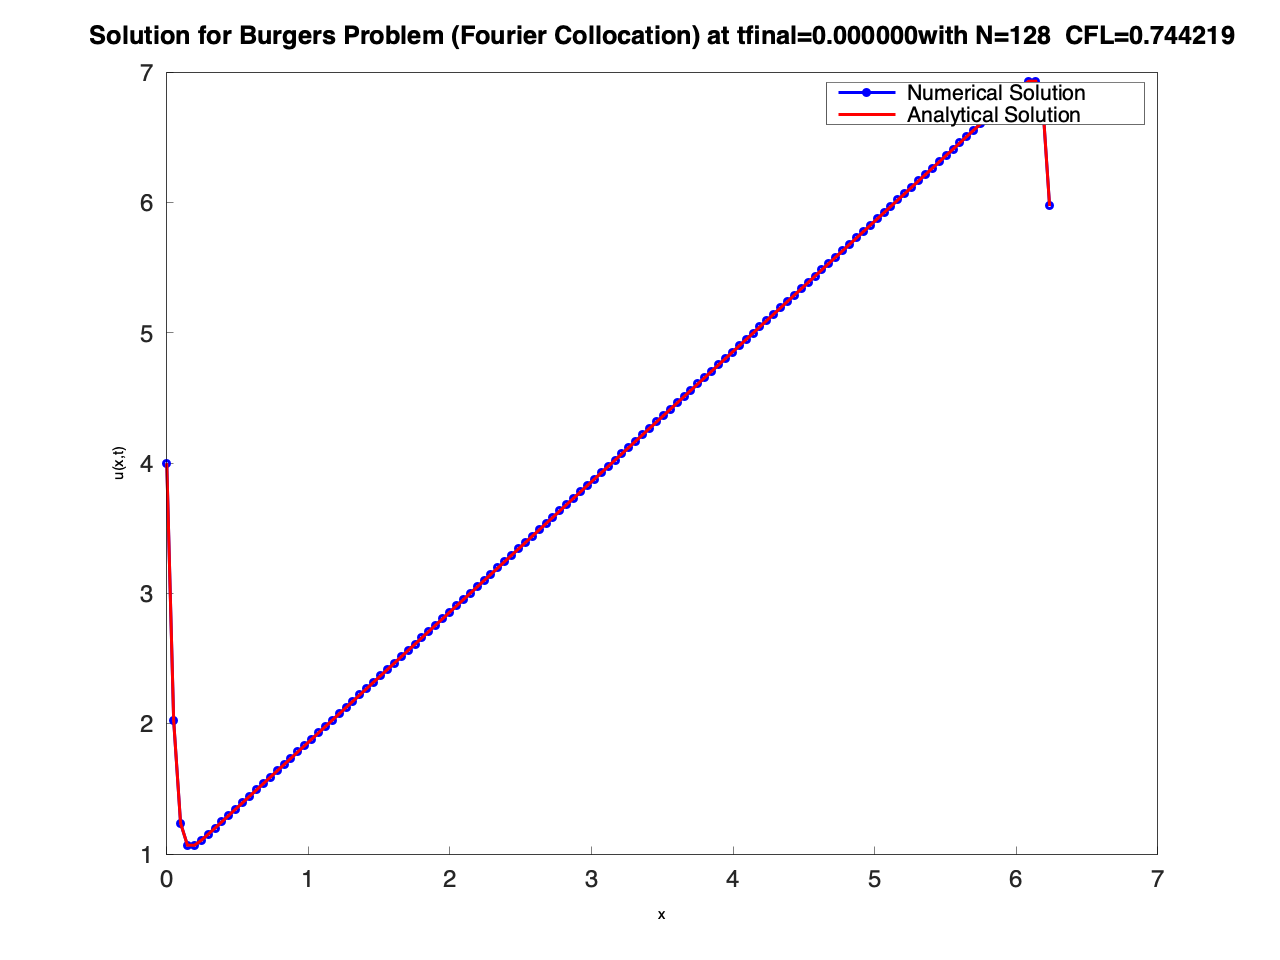
\includegraphics[width=\textwidth]{media/burger_tfinal_fc_128_0.000000.png}
		\caption{$t=0$}
		\label{sfig:sublabel1}
	\end{subfigure}%
	~
	\begin{subfigure}{0.5\textwidth}
		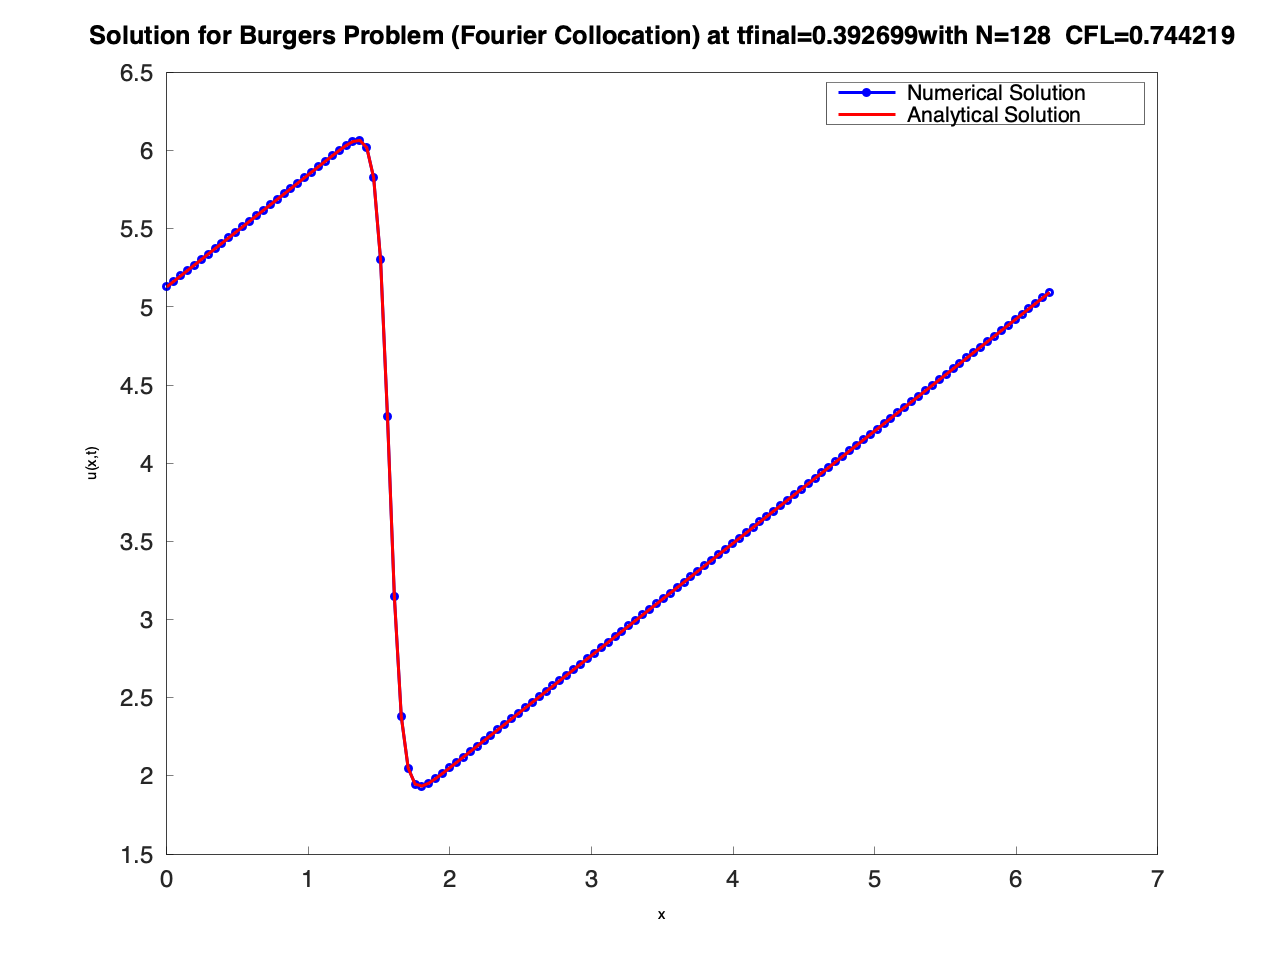
\includegraphics[width=\textwidth]{media/burger_tfinal_fc_128_0.392699.png}
		\caption{$t = \pi/ 8$}
		\label{sfig:sublabel2}
	\end{subfigure}\\
	\begin{subfigure}{0.5\textwidth}
		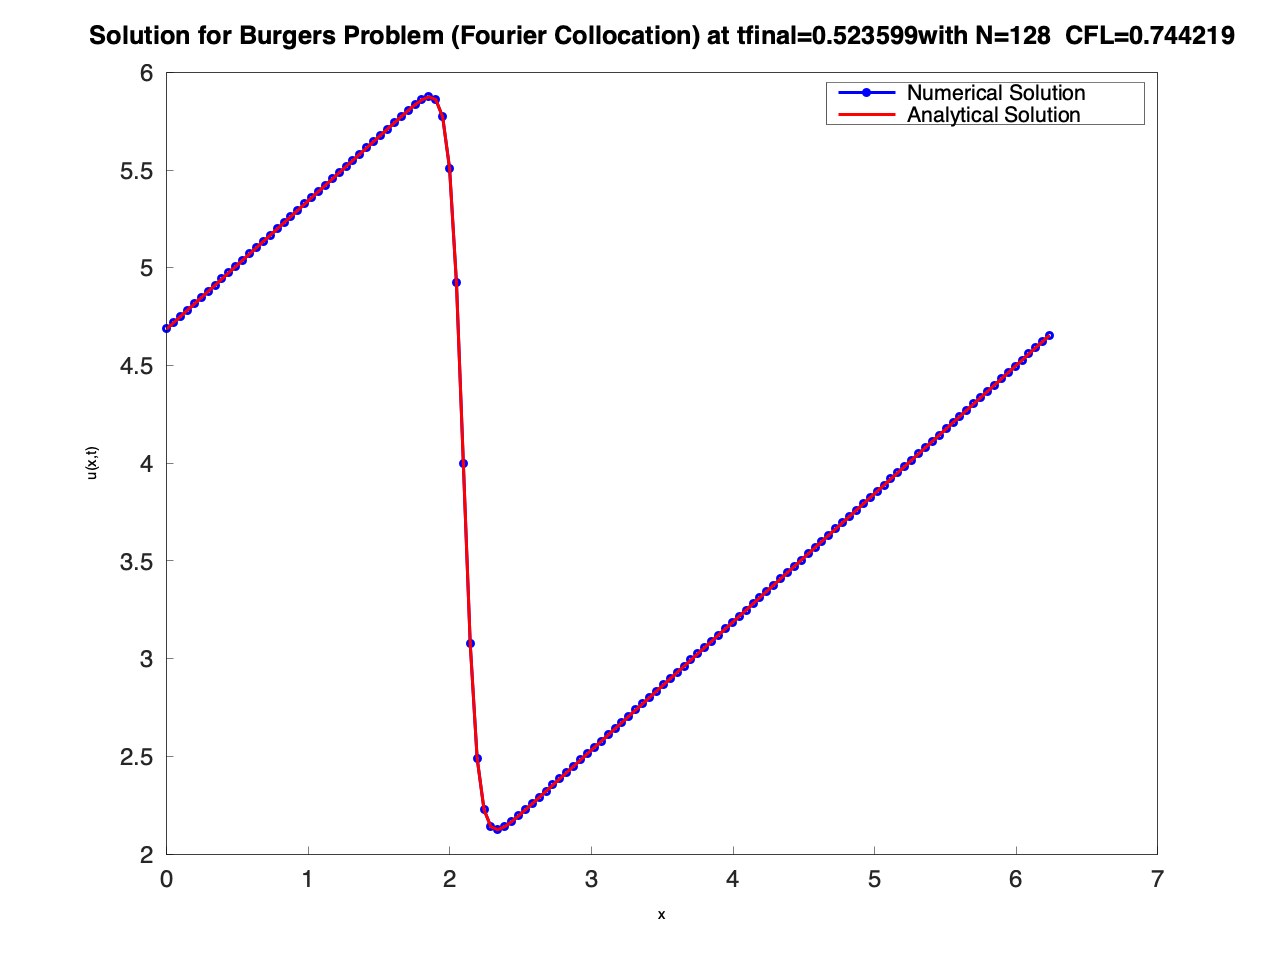
\includegraphics[width=\textwidth]{media/burger_tfinal_fc_128_0.523599.png}
		\caption{$t = \pi / 6$}
		\label{sfig:sublabel3}
	\end{subfigure}%
	~
	\begin{subfigure}{0.5\textwidth}
		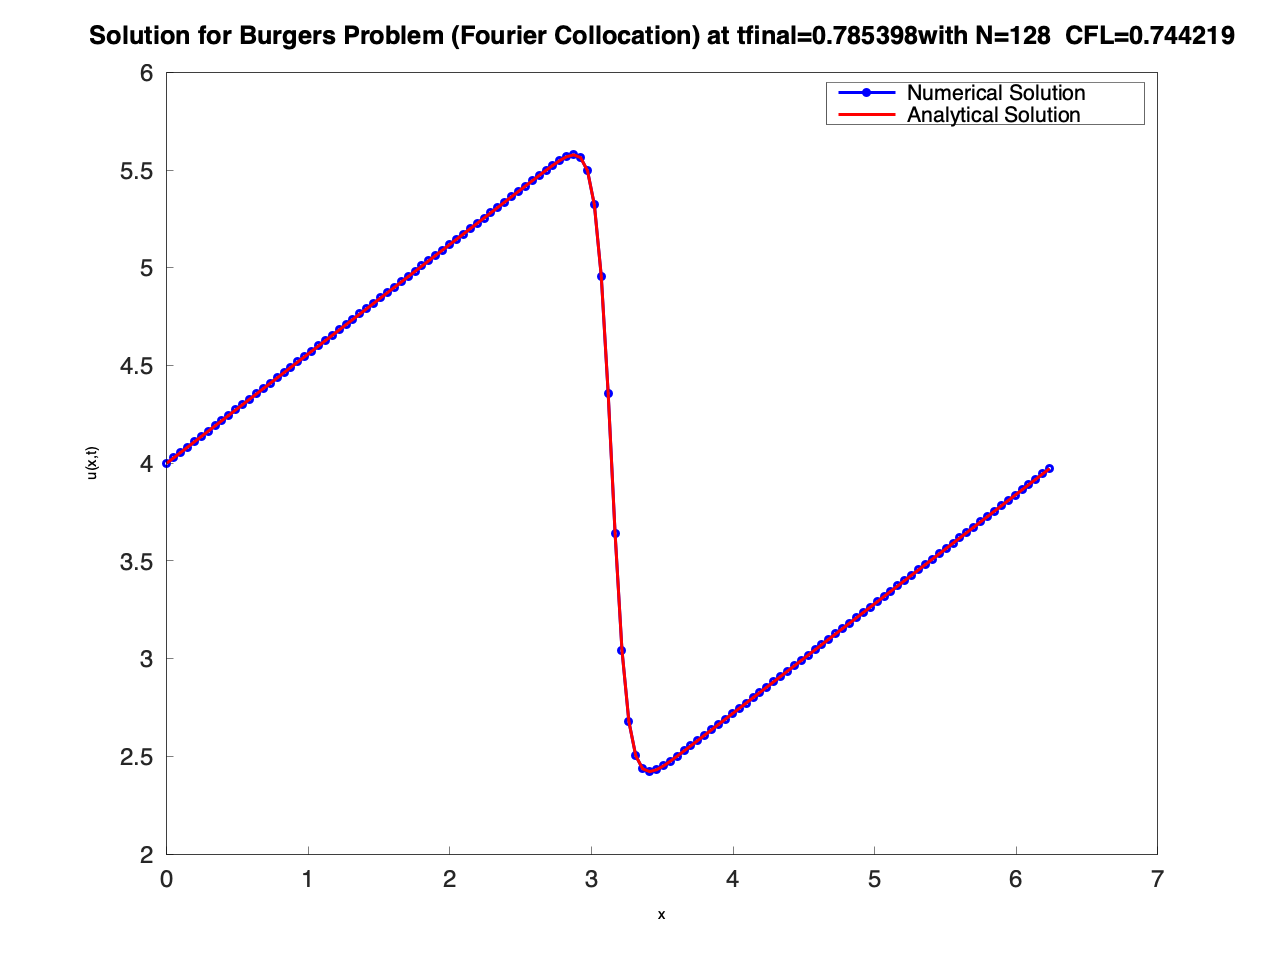
\includegraphics[width=\textwidth]{media/burger_tfinal_fc_128_0.785398.png}
		\caption{$t = \pi / 4$}
		\label{sfig:sublabel4}
	\end{subfigure}
	\caption{\textbf{Comparison of Analytical and Numerical Solution}
		The plots confirm excellent agreement between the numerical and analytical solutions at all time steps. The evolution shows the characteristic sawtooth-like traveling wave structure, with the solution maintaining its shape while propagating at velocity $c = 4.0$ and gradually smoothing due to viscous diffusion ($\nu = 0.1$). The perfect overlap between numerical and analytical solutions demonstrates the high accuracy of the Fourier Collocation method.
	}
	\label{fig:figureLabel}
\end{figure}

\subsubsection{Assessment of Overall Results}
The results from the Fourier Collocation implementation are \textbf{physically consistent and numerically sound}:

\begin{itemize}
	\item \textbf{Stability Analysis}: The CFL determination methodology successfully identifies stability boundaries through error spike detection
	\item \textbf{Convergence Validation}: Spectral convergence rates confirm optimal performance for smooth, periodic solutions
	\item \textbf{Physical Accuracy}: The decreasing error trend and excellent solution visualization validate the physical correctness of the implementation
	\item \textbf{Method Effectiveness}: The combination of Fourier spectral spatial discretization with 4th-order Runge-Kutta time integration provides both high accuracy and computational efficiency
\end{itemize}

\section{Solving Burger's equation using Fourier Galerkin}
In part 3  this section explores the Fourier Galerkin method for solving the Burgers' equation.
\begin{equation}
	\frac{\partial u(x, t)}{\partial t} + u(x, t) \frac{\partial u(x, t)}{\partial x} = \nu \frac{\partial^2 u(x, t)}{\partial x^2}
\end{equation}
with the same parameters ($c = 4.0$ and $\nu = 0.1$) and periodic boundary conditions on $x \in [0, 2\pi]$.\newline
The Fourier Galerkin method expands the solution in terms of Fourier modes:
\begin{equation}
	u(x, t) = \sum_{n=-N/2}^{N/2} \hat{u}_n(t)e^{inx}
\end{equation}
where $\hat{u}_n(t)$ are the time-dependent Fourier coefficients. Unlike the Collocation method which satisfies the PDE at specific grid points, the Galerkin method requires the residual to be orthogonal to each basis function, leading to a system of ODEs for the Fourier coefficients.
For the time integration, we used the same 4th-order Runge-Kutta scheme as in Part 2, but with a modified time step restriction:
\begin{equation}
	\Delta t \leq \text{CFL} \times \left[ \max_{x_j} \left(|u(x_j)| k_{max} + \nu (k_{max})^2  \right)\right]^{-1}
\end{equation}
where $k_{max} = N/2$ is the maximum wavenumber in the spectral representation.

\subsection{Determining Maximum CFL Values}

\subsection{Convergence Study}

\subsection{Comparison to Fourier Collocation}


\end{document}
